\documentclass[border=0pt]{standalone}

\usepackage{enumitem}

\usepackage[sc]{mathpazo}
\usepackage{tikz}
\linespread{1.05}

\newcommand\bluebullet{%
  \tikz[baseline=0ex]\fill[blue!75!black]
    (0,0)--(0.18,0.09)--(0,0.18)--cycle;}


\usepackage[table]{xcolor}
\definecolor{petrol}{RGB}{17,103,11}


\usepackage{tikz}
\usetikzlibrary{calc}


\usepackage{ragged2e}

\begin{document}
\small

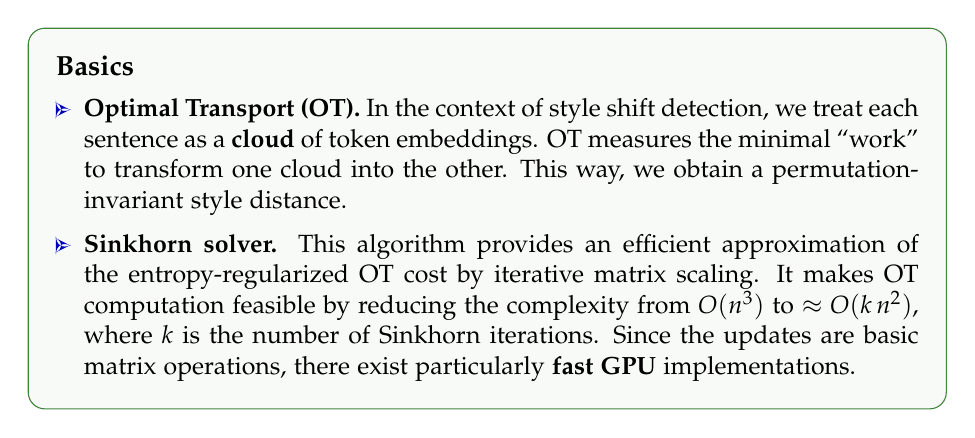
\begin{tikzpicture}
\node[
  draw=petrol!80,              
  fill=petrol!3,              
  rounded corners=6pt,
  minimum width=0.1\linewidth, 
  inner sep=10pt,               
  text width=0.95\linewidth-16pt, 
  font=\small,
  align=justify                
] (cap) {%
  \noindent {\normalsize\textbf{Basics}}
\begin{itemize}[label=\bluebullet,left=0em,itemsep=3pt]
  \item \textbf{Optimal Transport (OT).}  In the context of style shift detection, we treat each sentence as a \textbf{cloud} of token embeddings. OT measures the minimal ``work'' to transform one cloud into the other. This way, we obtain a permutation-invariant style distance.
  \item \textbf{Sinkhorn solver.}  This algorithm provides an efficient approximation of the entropy-regularized OT cost by iterative matrix scaling. It makes OT computation feasible by reducing the complexity from $O(n^3)$ to $\approx O(k\,n^2)$, where $k$ is the number of Sinkhorn iterations. Since the updates are basic matrix operations, there exist particularly \textbf{fast GPU} implementations. 
\end{itemize}
  };
\end{tikzpicture}

\end{document}